\begin{center}
	\begin{tabular}{M{9.25cm}M{8.75cm}}
		\textbf{TRƯỜNG THCS-THPT NGUYỄN KHUYẾN}& \textbf{ÔN TẬP KIỂM TRA CUỐI HỌC KÌ II}\\
		\textbf{MÃ ĐỀ: 001}& \textbf{Bài thi môn: VẬT LÝ 10}\\
		\textit{(Đề thi có 03 trang)}& \textit{Thời gian làm bài: 45 phút, không kể phát đề}
		
		\noindent\rule{4cm}{0.8pt} \\
	\end{tabular}
\end{center}
\setcounter{section}{0}
\section{Câu trắc nghiệm nhiều phương án lựa chọn}
\textit{Thí sinh trả lời từ câu 1 đến câu 12. Mỗi câu hỏi thí sinh chọn một phương án}
\setcounter{ex}{0}
\Opensolutionfile{ans}[ans/D10-CK2-001-TN]

% ===================================================================
\begin{ex}
	Khi con lắc đồng hồ dao động thì
	\choice
	{cơ năng của nó bằng không}
	{động năng và thế năng được chuyển hoá qua lại lẫn nhau nhờ công của lực căng dây treo}
	{\True động năng và thế năng được chuyển hoá qua lại lẫn nhau nhờ công của trọng lực}
	{động năng và thế năng được chuyển hoá qua lại lẫn nhau nhờ công của lực ma sát}
	\loigiai{}
\end{ex}
% ===================================================================
\begin{ex}
	Động lượng có đơn vị là
	\choice
	{\True \si{\newton\cdot\second}}
	{\si{\kilogram\cdot\meter/\second^2}}
	{\si{\newton\cdot\meter}}
	{\si{\newton/\second}}
	\loigiai{}
\end{ex}
% ===================================================================
\begin{ex}
	Nếu một xe đẩy va chạm hoàn toàn mềm với một xe đẩy đứng yên có khối lượng gấp đôi, thì chúng sẽ di chuyển bằng
	\choice
	{một nửa vận tốc ban đầu}
	{\True một phần ba vận tốc ban đầu}
	{gấp đôi vận tốc ban đầu}
	{gấp ba lần vận tốc ban đầu}
	\loigiai{}
\end{ex}

% ===================================================================
\begin{ex}
	Xe kéo dùng lực $\vec{F}$ có độ lớn \SI{800}{{\newton}} kéo một vật thì làm vật dịch chuyển một đoạn đường \SI{50}{\deci\meter} cùng hướng với lực kéo. Công của lực kéo thực hiện trên vật là
	\choice
	{\True \SI{4}{\kilo\joule}}
	{\SI{12}{\joule}}
	{\SI{5}{\kilo\joule}}
	{\SI{40}{\kilo\joule}}
	\loigiai{}
\end{ex}
% ===================================================================
\begin{ex}
	Động lượng của electron có khối lượng $\SI{9.1E-31}{\kilogram}$ và tốc độ $\SI{2.0E7}{\meter/\second}$ là
	\choice
	{\True $\SI{1.8E-23}{\kilogram\cdot\meter/\second}$}
	{$\SI{2.3E-23}{\kilogram\cdot\meter/\second}$}
	{$\SI{3.1E-23}{\kilogram\cdot\meter/\second}$}
	{$\SI{7.9E-23}{\kilogram\cdot\meter/\second}$}
	\loigiai{}
\end{ex}
% ===================================================================
\begin{ex}
	Một bóng đèn sợi đốt có công suất \SI{50}{\watt}, tiêu thụ năng lượng \SI{0.7}{\kilo\joule}. Thời gian thắp sáng bóng đèn là
	\choice
	{\SI{7}{\second}}
	{\SI{140}{\second}}
	{\True \SI{14}{\second}}
	{\SI{10}{\second}}
	\loigiai{}
\end{ex}
% ===================================================================
\begin{ex}
	Một ô tô có khối lượng \SI{1000}{\kilogram} đang chạy với tốc độ \SI{20}{\meter/\second} thì hãm phanh, giảm xuống đến tốc độ \SI{5}{\meter
		/\second}. Công của lực hãm tác dụng lên động cơ ô tô  trong quá trình hãm phanh là
	\choice
	{\SI{7.5}{\kilo\joule}}
	{\SI{187.5}{\kilo\joule}}
	{\True \SI{-187.5}{\kilo\joule}}
	{\SI{-7.5}{\kilo\joule}}
	\loigiai{}
\end{ex}
% ===================================================================
\begin{ex}
	Một bánh xe đang quay đều, mỗi phút nó quay được 3000 vòng. Phát biểu nào sau đây \textbf{sai} khi nói về chuyển động của bánh xe?
	\choice
	{Độ dịch chuyển góc của một điểm bất kì trên bánh xe (trừ những điểm thuộc trục quay) trong khoảng thời gian 0,01 giây bằng $\pi$ radian}
	{Những điểm cách trục quay \SI{10.0}{\centi\meter} thì có tốc độ $\xsi{10\pi}{\meter/\second}$}
	{\True Hai điểm bất kì trên bánh xe nếu cách nhau \SI{20.0}{\centi\meter} thì có tốc độ hơn kém nhau một lượng $\xsi{20\pi}{\meter/\second}$}
	{Những điểm càng xa trục quay thì gia tốc hướng tâm càng lớn}
	\loigiai{}
\end{ex}
% ===================================================================
\begin{ex}
	\immini{Một vật nhỏ chuyển động từ đỉnh A có độ cao \SI{3}{\meter} theo mặt phẳng nghiêng AB, sau đó chuyển động thẳng đứng lên trên đến C có độ cao cực đại \SI{4}{\meter}. Bỏ qua mọi ma sát, lấy $g=\SI{10}{\meter/\second^2}$. Độ lớn vận tốc ban đầu của vật tại A là
		\choice
		{\SI{7.7}{\meter/\second}}
		{$\xsi{5\sqrt{2}}{\meter/\second}$}
		{\True $\xsi{2\sqrt{5}}{\meter/\second}$}
		{\SI{8.9}{\meter/\second}}	
	}{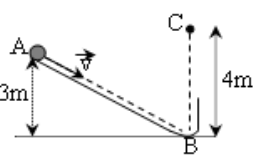
\includegraphics[scale=0.7]{../figs/D10-CK2-001-3}}
	
	\loigiai{}
\end{ex}
% ===================================================================
\begin{ex}
	Một vật khối lượng \SI{1}{\kilogram} chuyển động tròn đều với tốc độ \SI{10}{\meter/\second}. Độ biến thiên động lượng của vật sau $\dfrac{1}{4}$ chu kì kể từ lúc bắt đầu chuyển động bằng 
	\choice
	{\SI{20}{\kilogram\cdot\meter/\second}}
	{\SI{0}{\kilogram\cdot\meter/\second}}
	{\True $\xsi{10\sqrt{2}}{\kilogram\cdot\meter/\second}$}
	{$\xsi{5\sqrt{2}}{\kilogram\cdot\meter/\second}$}
	\loigiai{}
\end{ex}
% ===================================================================
\begin{ex}
	Một vật \SI{2}{\kilogram} rơi tự do xuống đất trong khoảng thời gian \SI{2}{\second} (lấy $g=\SI{9.8}{\meter/\second^2}$). Độ biến thiên động lượng của vật trong khoảng thời gian đó là
	\choice
	{\SI{40}{\kilogram\cdot\meter/\second}}
	{\SI{41}{\kilogram\cdot\meter/\second}}
	{\SI{38.3}{\kilogram\cdot\meter/\second}}
	{\True \SI{39.2}{\kilogram\cdot\meter/\second}}
	\loigiai{}
\end{ex}
% ===================================================================
\begin{ex}
	Có một bệ pháo khối lượng 10 tấn có thể chuyển động trên đường ray nằm ngang không ma sát. Trên bệ có gắn một khẩu pháo khối lượng 5 tấn. Giả sử khẩu pháo chứa một viên đạn khối lượng \SI{100}{\kilogram} và nhả đạn theo phương ngang với vận tốc đầu nòng \SI{500}{\meter/\second} (vận tốc đối với khẩu pháo). Biết bệ pháo chuyển động với tốc độ \SI{18}{\kilo\meter/\hour}. Nếu trước khi bắn, bệ pháo chuyển động cùng chiều bắn thì sau khi bắn bệ pháo chuyển động với vận tốc $\xsi{x}{(\meter/\second)}$. Nếu trước khi bắn, bệ pháo chuyển động ngược chiều bắn thì sau khi bắn bệ pháo chuyển động với vận tốc $\xsi{y}{(\meter/\second)}$. Chọn chiều chuyển động của pháo sau khi bắn làm chiều dương. Giá trị của $x-y$ gần nhất với giá trị nào sau đây?
	\choice
	{\True $10$}
	{$-7$}
	{$5$}
	{$-3$}
	\loigiai{}
\end{ex}
\Closesolutionfile{ans}
\section{Câu trắc nghiệm đúng/sai} 
\textit{Thí sinh trả lời từ câu 1 đến câu 4. Trong mỗi ý \textbf{a)}, \textbf{b)}, \textbf{c)}, \textbf{d)} ở mỗi câu, thí sinh chọn đúng hoặc sai}
\setcounter{ex}{0}\\
\Opensolutionfile{ans}[ans/D10-CK2-001-TF]
% ===================================================================
\begin{ex}
	Xét tính đúng/sai của các phát biểu sau:
	\choiceTF
	{\True Trong chuyển động tròn đều, vector gia tốc hướng tâm luôn hướng vào tâm quỹ đạo}
	{Gia tốc trong chuyển động tròn đều là kết quả của sự biến thiên về độ lớn của vận tốc}
	{\True Gia tốc hướng tâm có độ lớn $a_{\mathrm{ht}}=\dfrac{v^2}{R}$}
	{\True Vector gia tốc hướng tâm trong chuyển động tròn đều luôn vuông góc với vector vận tốc tại mọi thời điểm}
	\loigiai{}
\end{ex}
% ===================================================================
\begin{ex}
	Xét một vật nhỏ bắt đầu chuyển động trên một đường trượt không ma sát từ A đến C và sau đó trượt trên đường nằm ngang (có ma sát) từ C đến D.
	\immini{\choiceTF
		{\True Vật đạt tốc độ cực đại tại B}
		{\True Trong quá trình chuyển động từ C đến D, động năng của vật giảm}
		{Trong quá trình chuyển động từ A đến C, cơ năng của vật giảm}
		{\True Động năng của vật tại C bằng thế năng của vật tại A nếu chọn gốc thế năng tại C}}
	{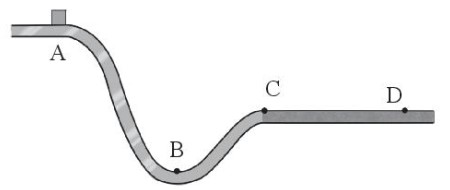
\includegraphics[scale=0.6]{../figs/D10-CK2-001-8}}
	\loigiai{}
\end{ex}
% ===================================================================
\begin{ex}
	Một vật có khối lượng $m_1=\SI{1}{\kilogram}$ chuyển động với vận tốc $v_1=\SI{3}{\meter/\second}$ đến va chạm với một vật có khối lượng $m_2=\SI{0.5}{\kilogram}$ đang đứng yên. Sau va chạm, hai vật dính vào nhau và chuyển động với cùng vận tốc.
	\choice
	{Do hai vật dính vào nhau nên động lượng của hệ giảm đi}
	{Tổng động năng của hệ trước và sau va chạm bằng nhau}
	{Động lượng của vật $m_1$ trước va chạm có độ lớn bằng \SI{4.5}{\kilogram\cdot\meter/\second}}
	{\True Tốc độ của hai vật sau va chạm bằng \SI{2}{\meter/\second}}
	\loigiai{}
\end{ex}
% ===================================================================
\begin{ex}
	Góc tạo bởi kim giờ và kim phút của một đồng hồ như hình bên.
	\immini{\choiceTF
		{Tại thời điểm trên hình, góc tạo bởi kim giờ và kim phút là $\SI{150}{\degree}$}
		{Sau 4 giờ, góc hợp bởi kim giờ và kim phút là $\SI{180}{\degree}$}
		{Kể từ thời điểm trên đến thời điểm 9 giờ, kim giờ đã quay được một góc bằng $\xsi{\dfrac{\pi}{3}}{\radian}$}
		{\True Khi kim phút quay được một vòng thì kim giờ quay được một góc $\xsi{\dfrac{\pi}{6}}{\radian}$}}
		{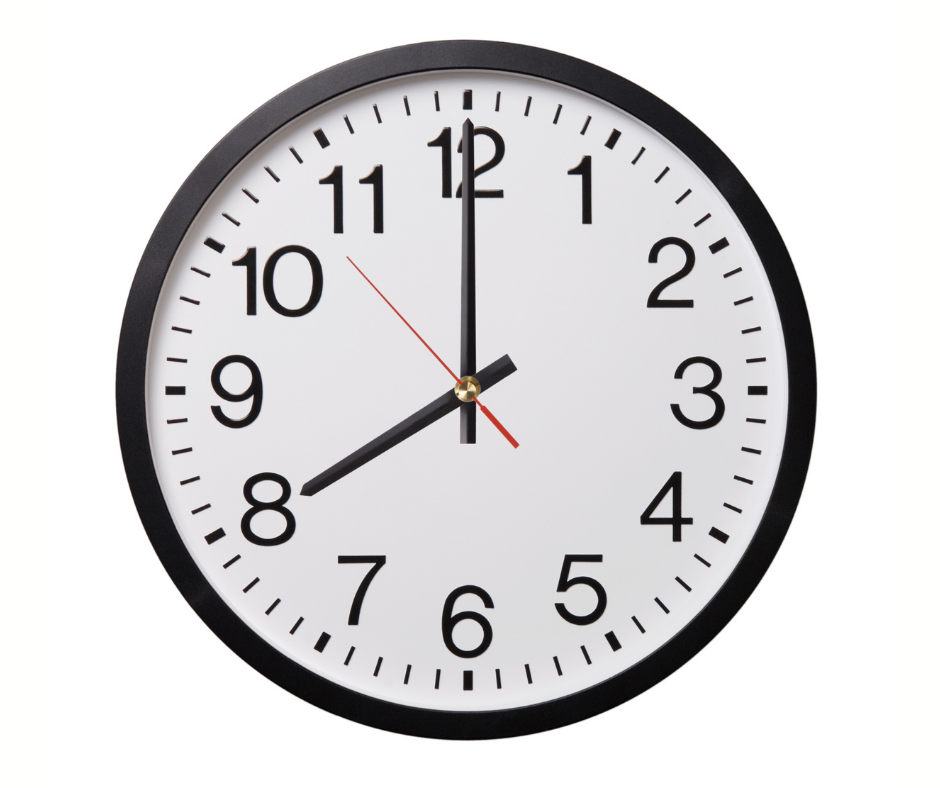
\includegraphics[scale=0.15]{../figs/D10-CK2-001-9}}
	\loigiai{\begin{itemchoice}
			\itemch Sai. Góc tạo bởi kim giờ và kim phút là $\SI{120}{\degree}$.
			\itemch Sai. Sau đó 4 giờ, kim giờ trùng với kim phút.
			\itemch Sai. Đến thời điểm 9 giờ, kim giờ quay được một góc bằng $\xsi{\dfrac{\pi}{6}}{\radian}$.
			\itemch Đúng. Kim phút quay một vòng thì kim giờ quay được $\dfrac{1}{12}$ vòng nên góc quay được là $\xsi{\dfrac{\pi}{6}}{\radian}$.
	\end{itemchoice}}
\end{ex}
\Closesolutionfile{ans}
\section{Tự luận} 
\setcounter{ex}{0}
\Opensolutionfile{ans}[ans/D10-CK2-001-TL]
% ===============================================================
\begin{ex}\textit{(1,0 điểm)}
	Một xe máy sử dụng lốp xe có đường kính bên ngoài (nơi tiếp xúc với mặt đường) là \SI{50}{\centi\meter} đang chuyển động thẳng đều. Hãy tính:
	\begin{enumerate}[label=\alph*)]
		\item Số vòng quay của lốp xe khi xe đi được quãng đường \SI{2}{\kilo\meter}.
		\item Tính tốc độ góc của 1 điểm trên lốp xe khi xe đang chạy với tốc độ \SI{72}{\kilo\meter/\hour}.
	\end{enumerate}
	\loigiai{
		
	}
\end{ex}
% ===============================================================
\begin{ex} \textit{(1,0 điểm)}
	\immini{Con lắc thử đạn là dụng cụ để đo tốc độ đầu đạn được bắn ra khỏi nòng súng với cấu tạo gồm một bao cát khối lượng $M=\SI{5.4}{\kilogram}$ được treo bằng hai sợi dây dài, nhẹ (xem hình vẽ bên). Ban đầu bao cát đứng yên. Một viên đạn khối lượng $m=\SI{9.5}{\gram}$ được bắn theo phương ngang với tốc độ ban đầu $v_0$ cắm chặt vào bao cát. Ngay sau đó, khối tâm của hệ viên đạn - bao cát bị đẩy lên cao một đoạn $h=\SI{6.5}{\centi\meter}$ theo phương thẳng đứng so với vị trí ban đầu của bao cát. Lấy gia tốc trọng trường $g=\SI{9.81}{\meter/\second}$.\\}
	{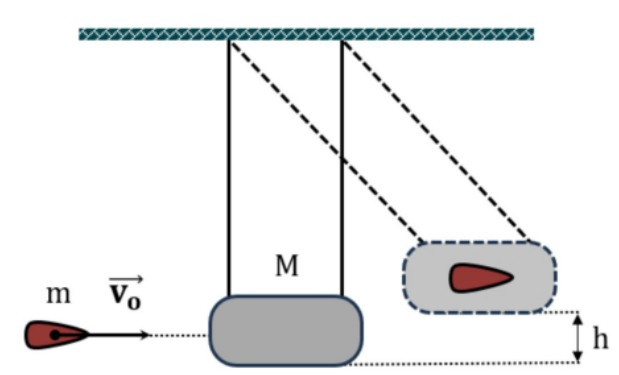
\includegraphics[scale=0.4]{../figs/D10-CK2-001-5}}
	 Bỏ qua lực cản không khí và xem rằng không có sự thất thoát năng lượng do tỏa nhiệt. Tính tốc độ $v_0$ ban đầu của viên đạn.
	\loigiai{
		
	}
\end{ex}
% ===============================================================
\begin{ex} \textit{(0,5 điểm)}
	\immini{Một đứa trẻ đang ở trên thuyền ném một gói hàng nặng \SI{5.3}{\kilogram} theo phương ngang với tốc độ \SI{10.0}{\meter/\second}. Hãy tính tốc độ của thuyền ngay sau khi ném, giả sử ban đầu thuyền đứng yên. Khối lượng của đứa trẻ là \SI{24}{\kilogram} và khối lượng của thuyền là \SI{35}{\kilogram}. Bỏ qua sức cản của nước. \textit{(Kết quả làm tròn đến chữ số hàng phần mười)}.}
	{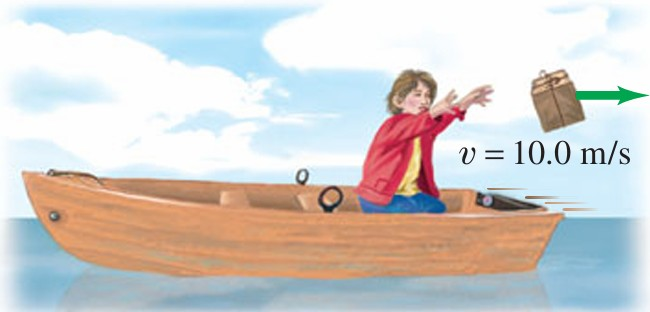
\includegraphics[scale=0.35]{../figs/D10-CK2-001-6}}
	\loigiai{
		
	}
\end{ex}
% ===============================================================
\begin{ex}\textit{(0,5 điểm)}
	\immini{Jack là một bạn trẻ năng động. Jack đang chạy với tốc độ \SI{6}{\meter/\second} thì bám vào một sợi dây dài \SI{10}{\meter} (dây không dãn và khối lượng dây không đáng kể) đang treo lơ lửng để đu người ra ngoài hồ và buông tay để rơi xuống hồ khi tốc độ bằng không. Góc $\theta$ tạo bởi dây và phương thẳng đứng lúc Jack buông tay là bao nhiêu độ? \textit{(Kết quả làm tròn đến chữ số hàng đơn vị)}.}
	{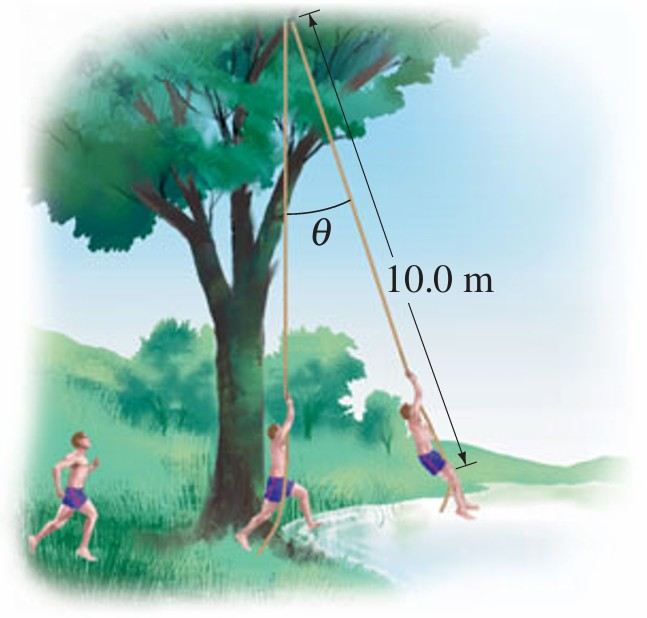
\includegraphics[scale=0.3]{../figs/D10-CK2-001-7}}
	\loigiai{
		
	}
\end{ex}
\Closesolutionfile{ans}
\begin{center}
	\textbf{--- TO BE CONTINUED \smiley ---}
\end{center}